\documentclass[9pt]{beamer}
% \documentclass[notes, handout, 9pt]{beamer}
% \documentclass[handout, 9pt]{beamer}

\usepackage{import}
\subimport{../}{preamble.tex}
\subimport{../}{beamer-theme.tex}
\usepackage{svg}

% Location for all figures / pictures
\graphicspath{{pictures/}{figures/}}

% % Figures inline
\usepackage{tikz}
\usepackage{pgfplots}
\usetikzlibrary{calc}
\usetikzlibrary{shapes.multipart}
\usetikzlibrary{decorations.pathreplacing}
\usetikzlibrary{arrows.meta}
\usepgfplotslibrary{fillbetween}

%--------------------------------------------------
% Presentation Information
%--------------------------------------------------
\title[Continuous Optimization]{Self-Concordant Functions}
\author[]{\textbf{Bart Van Parys}}
\date{Fall 2026}
%--------------------------------------------------

\begin{document}

\begin{frame}  

  \maketitle

  \vspace{-2em}
  
    \begin{center}
    \begin{tabular}{lll}
      Instructor : & \textbf{Bart Van Parys} & \textbf{(\href{mailto:mastermath@vanparys.xyz}{mastermath@vanparys.xyz})} \\
    \end{tabular}
  \end{center}
  
\end{frame}

\begin{frame}{Gradient versus Newton Method}

  Recall the reformulation of the gradient method
  \[
    x_{k+1 } \in \arg \min_{x} ~f(x_k) + \iprod{f'(x_k)}{x-x_k} + \frac{1}{2 h_k} \norm{x - x_k}^2_2. 
  \]

  \vfill

  Recall the reformulation of the Newton method
  \[
    x_{k+1 } \in \arg \min_{x} f(x_k) + \iprod{f'(x_k)}{x-x_k} + \frac{1}{2} \iprod{f''(x_k)(x - x_k)}{x - x_k}
  \]
  
\end{frame}

\begin{frame}{Newton's Method is Affine Invariant}


  
  \begin{minipage}{0.5\textwidth}

    Optimization Problem
    \[
      \begin{array}{rl}
        \min_{x\in \Re^n} & f(x)
      \end{array}
    \]

    \vfill

    Newton Iterates
    \[
      \begin{array}{rl}
        x_0 & = \bar x \\[0.5em]
              x_{k+1} & = x_k - f''(x_k)^{-1}f'(x_k)
      \end{array}
    \]

    \vfill

    \centering
    \includesvg[height=2.5cm]{conv1.svg}
  \end{minipage}%
  \hfill
  \begin{minipage}{0.5\textwidth}

    Optimization Problem
    \[
      \begin{array}{rl}
        \min_{y\in \Re^n} & \phi(y)\defn f(A y)
      \end{array}
    \]

    \vfill

    Newton Iterates
    \[
      \begin{array}{rl}
        y_0 & = A^{-1} \bar x \\[0.5em]
        y_{k+1} & = y_k - \phi''(y_k)^{-1}\phi'(y_k)
      \end{array}
    \]

    \vfill
    
    \centering
    \includesvg[height=2.5cm]{conv2.svg}
  \end{minipage}
  \vfill

  Invariance:
  \[
    \red{x_k\qquad=\qquad Ay_{k}}
  \]
\end{frame}


\begin{frame}{Kantorovich's Convergence Result is Not Affine Invariant !?}

  \begin{minipage}{0.7\textwidth}
    Let $f:\Re^n\to\nRe$ satisfy
    \begin{itemize}
      \setlength\itemsep{1em}
    \item $f$ is twice differentiable
    \item $f''(x^\star) \succeq \ell \cdot \mb I_n \succ 0$
    \item The Hessian $f''$ is Lipschitz continuous w.r.t.\ $\norm{\cdot}_2$, i.e.,
      \[
        \norm{f''(x) -f''(y)}\leq M \norm{x-y}_2
      \]
      where $\norm{A} = \sup_{\norm{x}_2\leq 1} \norm{A x}_2 = \max_i \abs{\lambda_i(A)}$.
    \end{itemize}    
  \end{minipage}%
  \hfill
  \begin{minipage}{0.3\textwidth}
    \centering
    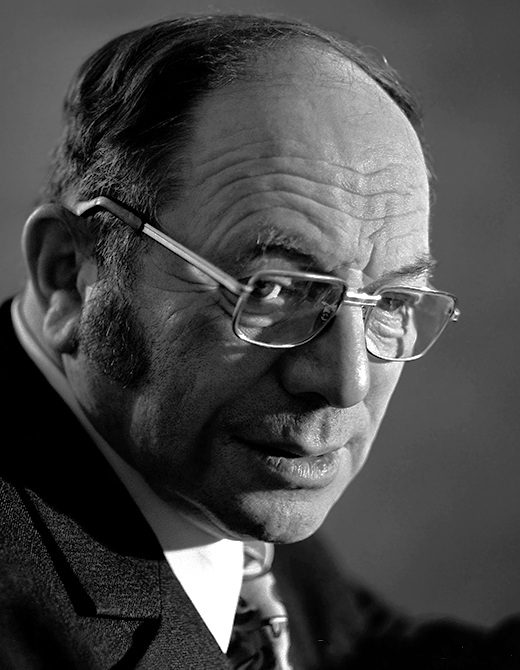
\includegraphics[height=3cm]{kantorovich.jpg}\\
    Kantorovich
  \end{minipage}

  \vfill
  
  \textbf{Theorem :} If \red{$\norm{x_0-x^\star}_2 \leq \frac{2\ell}{3 M}$}, then the iterates $x_k$ of Newton's method are \emph{well-defined} and
  \[
    \red{\Vert} x_{k+1}-x^\star \red{\Vert}_{\red{2}} \leq \frac{M \red{\Vert} x_k-x^\star \red{\Vert_2}^2}{2 \left( \ell - M \red{\Vert} x_k-x^\star \red{\Vert_2}\right)}\leq \frac{3M}{2 \ell} \red{\Vert} x_k-x^\star \red{\Vert_2}^2.
  \]
  
\end{frame}

\begin{frame}{The solution of Nesterov and Nemirovski:}

  Use the local norm $\norm{h}_x\defn \sqrt{\iprod{f''(x) h}{h}}$.\\[1em]

  Remark :
  \begin{itemize}
  \item $\norm{h}_{x, \star} = \sqrt{\iprod{f''(x)^{-1} h}{h}}$ \hfill \gray{Conjugacy}
  \item $\norm{h}_x = \sqrt{\iprod{\phi''(y) A^{-1} h}{A^{-1} h}}$ where $\phi(y) = f(Ay)$ \hfill \gray{Affine invariance}
  \end{itemize}
  
\end{frame}

\begin{frame}{Gradient versus Newton Method}

  Recall the reformulation of the gradient method
  \[
    x_{k+1 } \in \arg \min_{x} ~f(x_k) + \iprod{f'(x_k)}{x-x_k} + \frac{1}{2 h_k} \norm{x - x_k}^2_2. 
  \]

  \vfill

  The Newton method can be interpreted as
  \[
    x_{k+1 } \in \arg \min_{x} f(x_k) + \iprod{f'(x_k)}{x-x_k} + \frac{1}{2} \norm{x-x_k}^2_x.
  \]
  
\end{frame}


\section{Self-Concordant Functions}

\begin{frame}{Self-Concordant Functions}

  \textbf{Definition :} A \emph{LSC} function $f : \Re^n\to\nRe$ with \emph{open domain} $\dom(f)$ is \emph{self-concordant} if
  \[
    \exists M : ~ \forall x\in\dom(f),\, h\in \Re^n: \quad \abs{f'''(x)[h, h, h]}\leq M \norm{h}_x^3 = M\iprod{f''(x) h}{h}^{3/2}.
  \]

  \vfill

  \uncover<3->{
  \textbf{Example :} The function $f(t) = -\log(t)$. Indeed,
  \begin{itemize}
  \item $f'(t) = -\frac{1}{t}$,
  \item $f''(t) = \frac{1}{t^2}$,
  \item $f'''(t) = -\frac{2}{t^3}$.
  \end{itemize}
  We have $\norm{h}_t^2 = h^2/t^2$ and $\abs{f'''(t) [h, h, h]} = 2 h^3/t^3$. Thus $M=2$ would do.
}

  \vfill

  \textbf{Remark :}
  \begin{itemize}
  \item $f \in \mc{SC}(M) \implies f''(x) \succeq 0$, hence $f$ needs to be convex.
  \item<2-> The class of self-concordant functions will be those for which Newton's method ($\star$) works \emph{really} well.
  \end{itemize}
  
\end{frame}

\begin{frame}{Elementary Self-Concordant functions}

  The following functions are all self-concordant
  \begin{itemize}
    \setlength\itemsep{2em}
  \item Convex quadratic functions are in $\mc{SC}(0)$.
  \item $t>0 \mapsto -\log(t) \in \mc{SC}(2)$.
  \item $X\succ 0\mapsto -\log(\det(X)) \in \mc{SC}(2)$.
  \item<2-> $(t, x)\in L^n_{++}\defn\set{(x, t)}{t>\norm{x}_2} \mapsto -\log(t^2-\norm{x}^2_2) \in \mc{SC}(2)$
  \item<2-> $t\in(-\pi/2, \pi/2)\mapsto -\log(\cos(t)) \in \mc{SC}(2)$
  \end{itemize}
  
\end{frame}


\begin{frame}{Boundary Behavior}


  \textbf{Example:}
  
    \begin{center}
    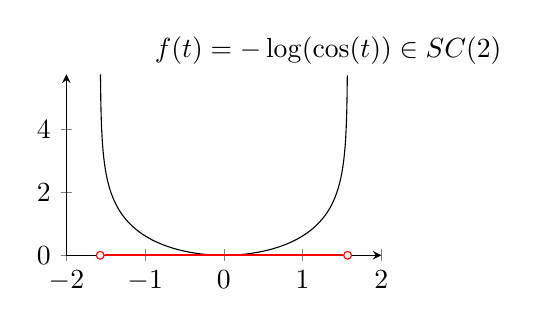
\begin{tikzpicture}
      
      \begin{axis}[
        %ticks=none,
        axis lines=left,
        y=0.4cm,            % y unit vector
        x=1cm,            % x unit vector
        clip=false,
        xmin =-2,
        xmax =2,
        %xlabel={ $\Re$},
        ylabel={ $f(t)=-\log(\cos(t))\in \mc{SC}(2)$},
        x label style={at={(axis description cs:0.9,0.05)},anchor=west},
        y label style={at={(axis description cs:0.25,1)},rotate=-90,anchor=south west},
        ]
        
        \addplot[mark=none, black, samples=1000, domain=-2:2] {-ln(cos(deg(x)))};

        \node[circle, inner sep=1, draw=red, fill=red!5] (a) at (axis cs:-1.5707963267948966, 0) {};
        \node[circle, inner sep=1, draw=red, fill=red!5] (b) at (axis cs:1.5707963267948966, 0) {};
        \draw[draw=red, thick] (a) -- (b);
        
      \end{axis}
      
    \end{tikzpicture}
  \end{center}

  \vfill

  \uncover<2->{
  \textbf{Theorem:} Let $f\in \mc{SC}(M)$ be a self-concordant function. Then for any sequence $x_k$ with limit $\bar x\in \cl(\dom(f))\setminus \dom(f)$ we have
  \[
    \lim_{k\to\infty} f(x_k) = +\infty.
  \]
  }
\end{frame}

\begin{frame}{Proof [$\star$]}

  \textbf{Proof:} Note that the sequence $\{f(x_k)\}$ is bounded from below due to the gradient inequality
  \[
    f(x_k)\geq f(x_0) + \iprod{f'(x_0)}{x_k-x_0}\implies \liminf_{k\to\infty } f(x_k) \geq f(x_0) + \iprod{f'(x_0)}{\bar x-x_0}=a.
  \]
  Assume that we have $f(x_k)\leq b<\infty$ is bounded from above for all $k$. There must exists an accumulation point $(\bar x, \bar f)$ with $\bar f\in [a, b]$ in the sequence $\{x_k, f(x_k)\}$. That is,
  $(x_{n_k}, f(x_{n_k})) \to (\bar x, \bar f)$
  for some sub-sequence $(x_{n_k}, f(x_{n_k}))$. However, $\bar x\not\in \dom(f)$ which is a contradiction with the fact that $f$ is LSC.
  
\end{frame}

\begin{frame}{Algebra of Self-Concordant Functions}

  Denote $f \in \mc{SC}(M)$ if $f$ is self-concordant with constant $M$.

  \vfill
  
  \textbf{Self-Concordance is invariant under :}
  \begin{itemize}
    \setlength\itemsep{1em}
  \item \emph{(Scaling)} $f \in \mc{SC}(M), ~\gamma\geq 0 \implies \gamma f\in \mc{SC}(M/\sqrt{\gamma})$. \\
    Therefore, we may consider \emph{$M\defn 2$} without much loss of generality.\\[1em]

  \item<2-> \emph{(Addition)} If $f \in \mc{SC}(M_f)$ and $g \in \mc{SC}(M_g)$, then $f+g \in \mc{SC}(\max(M_f, M_g))$. \\[1em]

  \item<3-> \emph{(Affine Transformations)} If $f \in \mc{SC}(M)$ and $A:\Re^n \to \Re^m$ is affine, then $f \circ A \in \mc{SC}(M)$.
  \end{itemize}

  \vfill

  \uncover<4->{
  \textbf{Illustration :} As $t\mapsto-\log(t) \in \mc{SC}(2)$, we have that $$x\mapsto -\textstyle\sum_i\log(a_i\tpose x - b_i) \in \mc{SC}(2).$$
  }
\end{frame}


\section{Why are self-concordant functions nice ?}

\begin{frame}{Example I}

  \begin{center}
    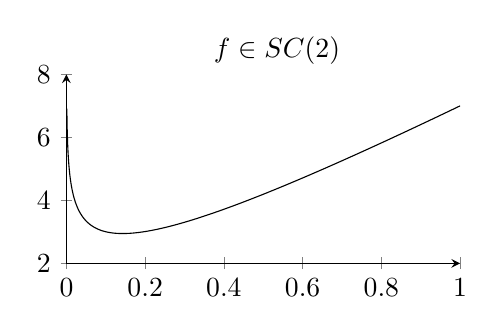
\begin{tikzpicture}
      
      \begin{axis}[
        %ticks=none,
        axis lines=left,
        y=0.4cm,            % y unit vector
        x=5cm,            % x unit vector
        clip=true,
        xmin =0,
        xmax =1,
        ymax=8,
        ymin=2,
        %xlabel={ $\Re$},
        ylabel={ $f\in \mc{SC}(2)$},
        x label style={at={(axis description cs:0.9,0.05)},anchor=west},
        y label style={at={(axis description cs:0.35,1)},rotate=-90,anchor=south west},
        ]
        
        \addplot[mark=none, black, samples=1000, domain=0:1] { 7*x-ln(x)};

      \end{axis}
      
    \end{tikzpicture}
  \end{center}

  \vfill
  
  \begin{itemize}
    \setlength\itemsep{1em}
  \item Convex function $f(x)=7x-\log x$ with minimizer $x^*=\frac{1}{7}=0.142857143$.
  \item Gradient $f'(x)=7-\frac{1}{x}$.
  \item Hessian $f''(x)=\frac{1}{x^2}$.
  \end{itemize}

\end{frame}

\begin{frame}{Computation}
  \begin{center}
    \begin{tabular}{|c||c||c||c|}
       \hline
       $k$ & $x_k$  &$x_k$ &$x_k$ \\ \hline
       0 & 1 &  0.01 & 0.1 \\
       1 & \red{-5}  & 0.0193 & 0.13 \\
       2 &  &  0.03599 & 0.1417 \\
       3 &  &  0.062917 & 0.14284777 \\
       4 &  &  0.098124 & 0.142857142\\
       5 &  &  0.128849782 &0.142857143\\
       6 & &  0.141483700 & 0.142857143\\
       7 & &  0.142843938 & 0.142857143\\
       8 & &  0.142857142 & 0.142857143\\\hline
     \end{tabular}
 \end{center}

 \vfill
 
 \textbf{Remarks:}
 \begin{itemize}
 \item When $\bold x_0\approx \bold x^\star$, then Newton's method converges.
 \item Failure I : If $\bold x_0 \not\approx \bold x^\star$, then Newton's method can fail to be defined.
 \end{itemize}
\end{frame}


\begin{frame}{An Ellipsoid Which is Always in $\dom(f)$}

  Let $f:\Re^n\to\nRe \in \mc{SC}(2)$ and $x\in \interior(\dom(f))$.

  \vfill

  \textbf{Theorem :} The \emph{Dikin ellipsoid} $B_x(x, 1) \defn \set{y\in\Re^n}{\norm{y-x}_x< 1}$ is contained in $\dom(f)$. \uncover<2->{Furthermore, when $y\in B_x(x, 1)$, then
    \[
      \frac{\norm{y-x}_{\red{x}}}{1+\norm{y-x}_{\red{x}}}  \leq \norm{y-x}_{\blue{y}} \leq \frac{\norm{y-x}_{\red{x}}}{1-\norm{y-x}_{\red{x}}}.
    \]
  }
  \vfill

  \begin{center}
    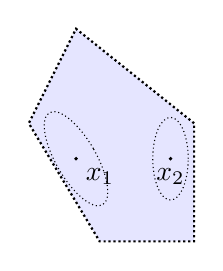
\begin{tikzpicture}[
      scale=1.5,
      % every node/.style={scale=1.5},
      ]

      \fill[draw=black, densely dotted, fill=blue!10, thick] (-1, 0) -- (-2, 0.8) -- (-2.4, 0) -- (-1.8, -1) -- (-1, -1) -- cycle;
      
  %     % \node[red, inner sep=1, fill, circle] (xstar) at (-2, 0.8) {};
  %     % \draw (-2.3, 0.8) -- (-1.7, 0.8) {};
  %     % \draw[->] (-2, 0.8) -- (-2, 1) {};
  %     % \node[above] at (-2, 0.95) {$-\bold c$}; 
      

      
      \node[black, inner sep=0.5, fill, circle] (x0) at (-2, -.3) {};
      \draw[black, rotate around={30:(x0)}, densely dotted] (x0) ellipse ({0.17} and {0.45});
      \node[below right, black] at (x0) {${x_1}$};

      \node[black, inner sep=0.5, fill, circle] (x1) at (-1.2, -.3) {};
      \draw[black, rotate around={0:(x1)}, densely dotted] (x1) ellipse ({0.15} and {0.35});
      \node[below, black] at (x1) {${x_2}$};

      
    \end{tikzpicture}
  \end{center}

  
\end{frame}

\begin{frame}{Proof I [$\star$]}

  Let us fix $x\in \interior(\dom(f))$ and $h\in \Re^n$ distinct from zero.
  Define the function $\phi(t) \defn \iprod{f''(x+th)h}{h}^{-1/2}$ with $\dom(\phi) = \set{t\in\Re}{x+th\in \dom f}$.

  \vspace{1em}

  \textbf{Lemma}:
  For all $t\in \dom (\phi)$ we have $\abs{\phi'(t)} \leq 1$.

  \vspace{1em}
  
  \textbf{Proof}:
  We have 
  \[
    -1 \leq \phi'(t) = -\frac{f'''(x+th)[h, h, h]}{2 \iprod{f''(x+th)h}{ h}^{3/2}}\leq 1
  \]
  for all $t\in \dom (\phi)$ as $f\in \mc{SC}(2)$.
  
  % We have  that $\phi(t)>0$ when $t\in \dom(\phi)$ as $f$ is convex.

  % Take now $h=y-x$ with $y\in B_x(x, 1)$. Then $\phi(0)>1$, and we have that
  % \(
  % \phi(0)-1 \leq \phi(1) \leq \phi(0)+1.
  % \)
  % It remains to simplify.
  
\end{frame}

\begin{frame}{Proof II [$\star$]}

  Let us fix $x\in \interior(\dom(f))$ and $h\in \Re^n$ distinct from zero.
  Define the function $\phi(t) \defn \iprod{f''(x+th)h}{h}^{-1/2}$ with $\dom(\phi) = \set{t\in\Re}{x+th\in \dom f}$.

  \vspace{1em}

  \textbf{Lemma}:
  We have \((-\phi(0), \phi(0)) \in \dom(\phi)\).

  \vspace{1em}
  
  \textbf{Proof}:
  We have  that $\phi(t)>0$ when $t\in \dom(\phi)$ as $f$ is convex.
  Since $f(x+ht)\to\infty$ as $x+ht$ approaches the boundary of $\dom(f)$ (See slide on boundary behavior), the function $\iprod{f''(x+th)h}{h}$ cannot remain bounded.
  Hence, $\dom(\phi) = \set{t}{\phi(t)>0}$. Note that $\abs{\phi'(t)}\leq 1$ implies that
  \[
    \phi(t) \geq \phi(0)-\abs{t}.
  \]
  
  % 

  % Take now $h=y-x$ with $y\in B_x(x, 1)$. Then $\phi(0)>1$, and we have that
  % \(
  % \phi(0)-1 \leq \phi(1) \leq \phi(0)+1.
  % \)
  % It remains to simplify.
  
\end{frame}


\begin{frame}{Proof III [$\star$]}

  \textbf{Part I:}
  From the previous it follows that
  \begin{align*}
    \dom(f) \supseteq & \set{x+th}{\exists h, ~\exists t\in (-\phi(0), \phi(0))}\\
    \supseteq &  \set{x+th}{\exists h, ~\exists t\in (-1/\norm{h}_x, 1/\norm{h}_x)} = B_x(x, 1).
  \end{align*}

  \textbf{Part II:}

  Take now $h=y-x$ with $y\in B_x(x, 1)$ and hence
  \(
  \phi(1) = \frac{1}{\norm{y-x}_y}
  \)
  and
  \(
  \phi(0) = \frac{1}{\norm{y-x}_x}.
  \)
  Here $\phi(0)>1$, and we have that
  \(
  \phi(0)-1 \leq \phi(1) \leq \phi(0)+1.
  \)
  It remains to simplify.
  
\end{frame}

\begin{frame}{Local Quadratic Upper Bound}

  \begin{center}
    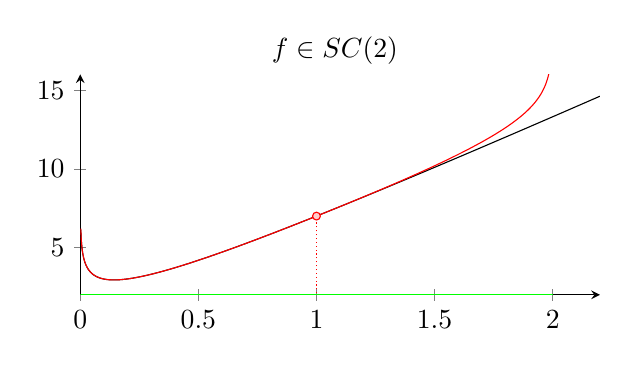
\begin{tikzpicture}
      
      \begin{axis}[
        % ticks=none,
        axis lines=left,
        y=0.2cm,            % y unit vector
        x=3cm,            % x unit vector
        clip=true,
        xmin =0,
        xmax =2.2,
        ymax=16,
        ymin=2,
        % xlabel={ $\Re$},
        ylabel={ $f\in \mc{SC}(2)$},
        x label style={at={(axis description cs:0.9,0.05)},anchor=west},
        y label style={at={(axis description cs:0.35,1)},rotate=-90,anchor=south west},
        ]
        
        \addplot[mark=none, black, samples=1000, domain=0:2.2] { 7*x-ln(x)};
        \addplot[mark=none, red, samples=1000, domain=0:2.2] { 7+6*(x-1)-((x-1)*1*(x-1))^(0.5)-ln(1-((x-1)*1*(x-1))^(0.5))};

        \node[circle, draw=red, fill=red!20, inner sep=1] (f0) at (axis cs:1, 7) {};
        \node[] (x0) at (axis cs:1, 0) {};
        \draw[densely dotted, draw=red] (x0) -- (f0);

        \draw[draw=green, thick] (axis cs:0, 2) -- (axis cs:2, 2);
        
      \end{axis}
      
    \end{tikzpicture}
  \end{center}

  \vfill

  \textbf{Theorem:} Let $f \in \mc{SC}(2)$ and $r\defn \norm{y-x}_x\defn \sqrt{(y-x) f''(x) (y-x)}<1$, then
  $$f(y) \leq f(x) + \iprod{f'(x)}{y-x} \red{- r - \log(1-r)}.$$

  \vfill

  \textbf{Note:} We have the Taylor expansion
  \[
    - r - \log(1-r) = r^2/2 + \mc O(r^3)
  \]
  
\end{frame}

\begin{frame}{Proof [$\star$]}

    \textbf{Proof [$\star$]:} Let us denote $x(t)=x+(y-x)t$. We have
  \[
    \begin{array}{rl}
      \iprod{f'(y)-f'(x)}{ y-x} & = \int_0^1 \iprod{f''(x+(y-x)t)(y-x)}{y-x}\d t\\[0.5em]
                                & = \int_0^1 \frac{1}{t^2} \norm{x(t)-x}_{x(t)}^2\d t\leq \int_0^1 \frac{r^2}{(1-tr)^2} \d t = r^2/(1-r).
    \end{array}
  \]
  using the inequality $\norm{x(t)-x}_{x(t)}\leq \frac{\norm{x(t)-x}_{x}}{1-\norm{x(t)-x}_{x}}$.
  Further, we obtain
  \[
    \begin{array}{rl}
      & f(y) - f(x) - \iprod{f'(x)}{ y-x}\\[0.5em]
      = &  \int_0^1 \iprod{f'(x+(y-x)t)-f'(x)}{ y-x}\d t\\[0.5em]
      = &\int_0^1 \iprod{f'(x+(y-x)t)-f'(x)}{ (x(t)-x)/t} \d t\\[0.5em]
      \leq & \int_0^1 r^2t/(1-rt)\d t = -r-\log(1-r).
    \end{array}
  \]

\end{frame}


\begin{frame}{Local Quadratic Lower Bound}

  \begin{center}
    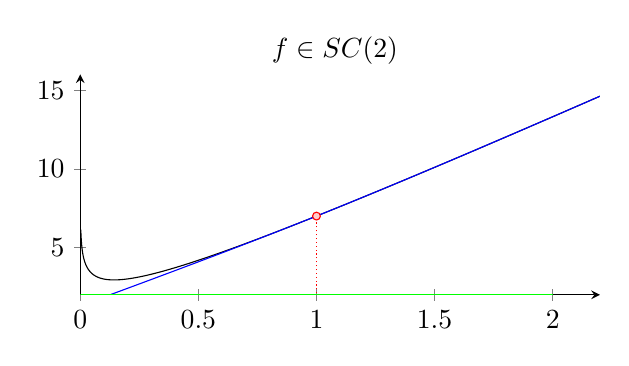
\begin{tikzpicture}
      
      \begin{axis}[
        % ticks=none,
        axis lines=left,
        y=0.2cm,            % y unit vector
        x=3cm,            % x unit vector
        clip=true,
        xmin =0,
        xmax =2.2,
        ymax=16,
        ymin=2,
        % xlabel={ $\Re$},
        ylabel={ $f\in \mc{SC}(2)$},
        x label style={at={(axis description cs:0.9,0.05)},anchor=west},
        y label style={at={(axis description cs:0.35,1)},rotate=-90,anchor=south west},
        ]
        
        \addplot[mark=none, black, samples=1000, domain=0:2.2] { 7*x-ln(x)};
        %\addplot[mark=none, red, samples=1000, domain=0:2.2] { 7+6*(x-1)-((x-1)*1*(x-1))^(0.5)-ln(1-((x-1)*1*(x-1))^(0.5))};
        \addplot[mark=none, blue, samples=1000, domain=0:2.2] { 7+6*(x-1)+((x-1)*1*(x-1))^(0.5)-ln(1+((x-1)*1*(x-1))^(0.5))};

        \node[circle, draw=red, fill=red!20, inner sep=1] (f0) at (axis cs:1, 7) {};
        \node[] (x0) at (axis cs:1, 0) {};
        \draw[densely dotted, draw=red] (x0) -- (f0);

        \draw[draw=green, thick] (axis cs:0, 2) -- (axis cs:2, 2);
        
      \end{axis}
      
    \end{tikzpicture}
  \end{center}

  \vfill

  \textbf{Theorem:} Let $f \in \mc{SC}(2)$ and $r\defn \norm{y-x}_x\defn \sqrt{(y-x) f''(x) (y-x)}$, then
  $$f(y) \geq f(x) + \iprod{f'(x)}{y-x} \blue{+ r - \log(1+r)}.$$

  \vfill

  \textbf{Note:} We have the Taylor expansion
  \[
     r - \log(1+r) = r^2/2 + \mc O(r^3)
  \]
  
\end{frame}

\begin{frame}{Proof [$\star$]}

  \textbf{Proof [$\star$]:} Let us denote $x(t)=x+(y-x)t$. We have
  \[
    \begin{array}{rl}
      \iprod{f'(y)-f'(x)}{ y-x} & = \int_0^1 \iprod{f''(x+(y-x)t)(y-x)}{y-x}\d t\\[0.5em]
                                & = \int_0^1 \frac{1}{t^2} \norm{x(t)-x}_{x(t)}^2\d t\geq \int_0^1 \frac{r^2}{(1+tr)^2} \d t = r^2/(1+r).
    \end{array}
  \]
  using the inequality $\norm{x(t)-x}_{x(t)}\geq \frac{\norm{x(t)-x}_{x}}{1+\norm{x(t)-x}_{x}}$.
  Further, we obtain
  \[
    \begin{array}{rl}
      & f(y) - f(x) - \iprod{f'(x)}{ y-x}\\[0.5em]
      = &  \int_0^1 \iprod{f'(x+(y-x)t)-f'(x)}{ y-x}\d t\\[0.5em]
      = &\int_0^1 \iprod{f'(x+(y-x)t)-f'(x)}{ (x(t)-x)/t} \d t\\[0.5em]
      \geq & \int_0^1 r^2t/(1+rt)\d t = r-\log(1+r).
    \end{array}
  \]

  
\end{frame}

\begin{frame}{The Hessian is Very ``Smooth''}

  In Kantorovich's proof concerning the convergence of Newton's method, it was assumed that $f''$ does not vary too abruptly. We assumed in fact the Lipschitz condition
  \[
    \norm{f''(y) -f''(x)} \leq M \norm{y-x}_2.
  \]
  We have the something similar for self-concordant functions, but the bounds are far better!

  \vfill

  \textbf{Theorem :} Let $f\in \mc{SC}(2)$, $x \in \dom(f)$ and $y \in B_x(x, 1)$. Let $r\defn\norm{y-x}_x$. Then
  \[
    (1-r)^2 f''(x) \preceq f''(y) \preceq f''(x)/(1-r)^2.
  \]
  
\end{frame}


\begin{frame}{The Proof is Not Completely Straightforward $[\star]$}


  \textbf{Proof :} Let $x \in \interior(\dom(f))$ and $h$ distinct from zero. Let
  \[
     \phi(t) \defn \iprod{f''(x+t(y-x))h}{h} = \iprod{f''(x_t)h}{h} ~~t\in [0,1]
  \]
  We have that
  \[
    \begin{aligned}
      \phi'(t) \leq \abs{\phi'(t)} & = \abs{f'''(x+t(y-x))[y-x, h, h]} \leq 2 \norm{y-x}_{x_t} \norm{h}_{x_t}^2 \leq 2 \norm{y-x}_{x_t} \phi(t)\\
      \abs{\phi'(t)}/\phi(t) & \leq \frac 2t \norm{x_t-x}_{x_t} \blue{\leq} \frac2t \frac{\norm{x_t-x}_x}{1-\norm{x_t-x}_x} = 2\frac{\norm{y-x}_x}{1-t\norm{y-x}_x} = \frac{2r}{1-tr}
    \end{aligned}
  \]
  by using the result $\norm{x_t-x}_{x_t}\leq \norm{x_t-x}_x/(1-\norm{x_t-x}_x)$. 
  Thus
  \[
    2[\log(1-tr)]' = -\frac{2 r}{1-tr} \leq \frac{\phi'(t)}{\phi(t)} = [\log(\phi(t))]'\leq \frac{2 r}{1-tr} = -2[\log(1-tr)]'.
  \]
  Integrating on $[0, 1]$ we get both inequalities. 
\end{frame}


\section{Damped Newton's Method}

\begin{frame}{Damped Newton Method}
  
  The damped Newton Method minimizes in each iteration the upper bound
  \[
    \begin{array}{rl}
      (x_{k+1}, r_{k+1}) \defn \min_{x, r} & f(x_k) + \iprod{f'(x_k)}{x-x_k} - r - \log(1-r)\\[0.5em]
      \st & r = \sqrt{\iprod{f''(x_k)(x-x_k)}{ x-x_k}}.
    \end{array}
  \]
  The optimization problem can be solved closed form!

  \vfill

  \uncover<2->{
  \begin{algorithm}[H]
    \SetKwInput{Initialization}{Initialisation}
    \Initialization{$x_0\in \dom(f)$}
    \For{$k\geq 0$}{
      $\lambda(x_k) = \norm{f'(x_k)}_{x_k, \star}\gray{=\sqrt{\iprod{f''(x_k)^{-1}f'(x_k)}{f'(x_k)}}}$\\
      $x_{k+1} \defn x_k - \frac{1}{\lambda(x_k)+1} f''(x_k)^{-1} f'(x_k)$ 
    }
    \caption{\emph{Damped Newton Method}}
  \end{algorithm}
  }

\end{frame}


\begin{frame}{Damped Newton Method}
  

  \vfill
  
  The \emph{damped} Newton method is a \emph{global} descent method!

  \vfill
  
  \textbf{Proof :}
  \begin{itemize}
  \item Note that $r_{k+1}=\norm{x_{k+1}-x_k}_{x_k} = \lambda(x_k)/(1+\lambda(x_k)) < 1$. Thus, $x_{k+1} \in B_{x_k}(x_k, 1) \subseteq \dom(f)$.
  \item Using our upper bound we get
    \begin{align*}
      & f(x_{k+1})\\[0.5em]
       \leq & f(x_k) + \iprod{f'(x_k)}{x_{k+1}-x_k} - \lambda(x_k)/(1+\lambda(x_k)) - \log(1- \lambda(x_k)/(1+\lambda(x_k)))\\[0.5em]
      \leq & f(x_k) -\lambda(x_k)^2/(1+\lambda(x_k)) - \lambda(x_k)/(1+\lambda(x_k)) + \log(1+\lambda(x_k))\\[0.5em]
      \leq & f(x_k) - \lambda(x_k) + \log(1+\lambda(x_k)) \leq f(x_k)
    \end{align*}
  \end{itemize}
\end{frame}


\begin{frame}{The Newton Decrement}

  Let $\lambda(x) \defn \norm{f'(x)}_{x, \star}$ be the \emph{Newton decrement}. Newton decrement is a good measure of suboptimality.

  \vfill

  \textbf{Theorem :} Let $\lambda(x)<1$. Then,
  \[
    f(x)-f(x^\star) \leq  -\lambda(x) - \log(1-\lambda(x))
  \]
  and
  \[
    \norm{x-x^\star}_x \leq \frac{\lambda(x)}{1-\lambda(x)}. 
  \]

\end{frame}

\begin{frame}{Proof [$\star$]}

  \textbf{Proof:} We will prove that for any two points $x$ and $y$ with $\norm{f'(y)-f'(x)}_{y, \star}<1$ we have
  \[
    f(y) \leq f(x) + \iprod{f'(x)}{y-x} + \omega_\star(\norm{f'(y)-f'(x)}_{y, \star})
  \]
  with $\omega_\star: r\mapsto -r-\log(1-r)$. The claim then follows by taking $x=x^\star$ and $y=x_k$ and noting that $f'(x^\star)=0$.
%
  Consider a self-concordant function
  \(
    \phi(z) = f(z)-\iprod{f'(x)}{z}
  \)
  with $\phi'(x)=0$. Hence, we have
  \begin{align*}
    f(x) -\iprod{f'(x)}{x} & = \phi(x) = \min_z \phi(z) \\[0.5em]
                           & \geq \min_z \phi(y) +\iprod{\phi'(y)}{z-y}+\omega(\norm{z-y}_y) \\[0.5em]
                           & = \phi(y) - \max_\lambda  \iprod{-\phi'(y)}{\lambda}-\omega(\norm{\lambda}_y) \\[0.5em]
                           & =  \phi(y) -\omega_\star(\norm{-\phi'(y)}_{y, \star}) = \phi(y) -\omega_\star(\norm{\phi'(y)}_{y, \star}) \\[0.5em]
                           & = f(y) - \iprod{f'(x)}{y} - \omega_\star(\norm{f'(y)-f'(x)}_{y, \star})
  \end{align*}
  with $\omega:s\mapsto s-\log(1+s)$ the conjugate of $\omega_\star$.
\end{frame}

\begin{frame}{Proof [$\star$]}

  \textbf{Proof:}
  For any two points $x$ and $y$ with $\norm{y-x}_x$ we have shown in the proof of the lower bound that
  \(
    \iprod{f'(y)-f'(x)}{y-x} \geq \norm{y-x}_x^2/(1+\norm{y-x}_x).
  \)
  Applying this inequality at $y=x$ and $x=x^\star$ gives us
  \(
    \iprod{f'(x)}{x-x^\star} \geq r^2/(1+r)
    \)
    as we have $f'(x^\star)=0$.
  Cauchy-Schwarz gives us the inequality
  \begin{align*}
    &r^2/(1+r)\leq \iprod{f'(x)}{ x-x^\star} \leq \norm{f'(x)}_{x, \star}\norm{x-x^\star}_x = \lambda(x)r\\[0.5em]
    \implies & r=\norm{x-x^\star}_x\leq \frac{\lambda(x)}{1-\lambda(x)}.
  \end{align*}
  
\end{frame}

\begin{frame}{Quadratic Convergence Zone of Newton Method}


   \begin{algorithm}[H]
    \SetKwInput{Initialization}{Initialisation}
    \Initialization{$x_0\in \dom(f)$}
    \For{$k\geq 0$}{
      $x_{k+1} \defn x_k - f''(x_k)^{-1} f'(x_k)$ 
    }
    \caption{\emph{Standard Newton's method}}
  \end{algorithm}

  \vfill
  
  \textbf{Theorem :} Assume that $\lambda(x_k)<1$. Then,
  \[
    \lambda(x_{k+1}) \leq \frac{\lambda(x_k)^2}{(1-\lambda(x_k))^2}.
  \]

  In particular, if $\lambda(x_k) < \frac{3-\sqrt{5}}{2} \approx 0.3819$, then \emph{$\lambda(x_{k+1})<\lambda(x_k)$}.
 
\end{frame}

\begin{frame}{Drawing}

  \begin{center}
    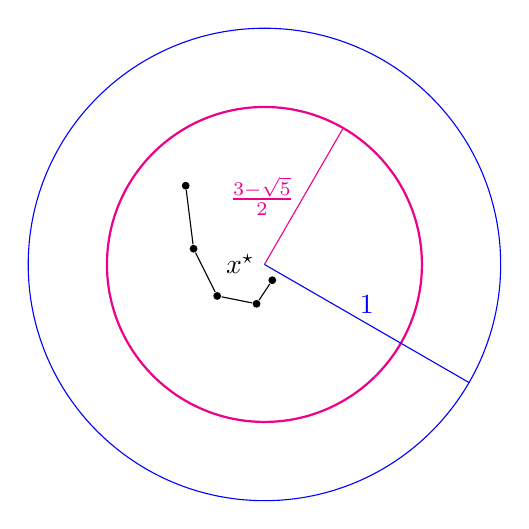
\begin{tikzpicture}
      \draw [magenta, thick] circle [radius=2];
      \draw [blue] circle [radius=3];

      \draw [magenta] (0,0) -- node[left,magenta] {$\frac{3-\sqrt{5}}{2}$} (60:2);
      \node [left] at (0, 0) {$x^\star$};

      \draw [blue] (0,0) -- node[above,blue] {$1$} (-30:3);

      \node [fill=black,inner sep=1, circle] (x0) at (-1, 1) {};
      \node [fill=black,inner sep=1, circle] (x1) at (-0.9, 0.2) {};
      \node [fill=black,inner sep=1, circle] (x2) at (-0.6, -0.4) {};
      \node [fill=black,inner sep=1, circle] (x3) at (-0.1, -0.5) {};
      \node [fill=black,inner sep=1, circle] (x4) at (0.1, -0.2) {};

      \draw (x0)--(x1);
      \draw (x1)--(x2);
      \draw (x2)--(x3);
      \draw (x3)--(x4);
    
  \end{tikzpicture}
\end{center}

\end{frame}


\begin{frame}{Proof [$\star$]}

  \textbf{Proof :} Let $r_k\defn \norm{x_{k+1}-x_k}_{x_k}$. Then $\lambda(x_k)=r_k<1$. We have
  \[
    \lambda(x_{k+1})^2 = \iprod{f''(x_{k+1})^{-1} f'(x_{k+1})}{f'(x_{k+1})} \leq \frac{1}{(1-r_k)^2} \iprod{f''(x_k)^{-1} f'(x_{k+1})}{f'(x_{k+1})}.
  \]
  Things are about to become technical. First,
  \[
    f'(x_{k+1}) = f'(x_{k+1})-f'(x_k) - f''(x_k)(x_{k+1}-x_k) = G(x_{k+1}-x_k),
  \]
  where
  \[
    f''(x_k) \left(\frac{r_k^2}{3}-r_k\right) \preceq G = \int_0^1 \left[f''(x_k + t (x_{k+1}-x_k))-f''(x_k)\right] dt \preceq f''(x_k)\frac{r_k}{1-r_k}
  \]
  as a consequence of the smoothness of the Hessian. Since $r_k^2/3-r_k \leq \tfrac{r_k}{(1-r_k)}$, we get
  \[
    \lambda(x_{k+1})^2 = \norm{f'(x_{k+1})}^2_{x_k, \star} \leq \frac{r_k^2}{(1-r_k)^4} \iprod{f''(x_k)^{-1} f'(x_k)}{f'(x_k)}=\frac{r_k^2\lambda(x_k)^2}{(1-r_k)^4}.
  \]
\end{frame}


\begin{frame}{Overall Algorithm}


  \begin{algorithm}[H]
    \SetKwInput{Initialization}{Initialisation}
    \Initialization{$x_0\in \dom(f)$, $\beta<(3-\sqrt{5})/2$}
    \For{$k\geq 0$}{
      $\lambda(x_k)=\norm{f'(x_k)}_{x_k, \star}$\\
      \If{$\lambda_k\geq \beta$}{
        $x_{k+1} \defn x_k - \frac{1}{\lambda(x_k)+1} f''(x_k)^{-1} f'(x_k)$
      }
      \Else{
        $x_{k+1} \defn x_k - f''(x_k)^{-1} f'(x_k)$
      }      
    }
    \caption{\emph{Newton switching method}}
  \end{algorithm}
  
  \vfill

  \textbf{Convergence:}
  \begin{itemize}
  \item If $\lambda(x_k) \geq \beta$, use the damped Newton method. We can guarantee $f(x_{k+1}) \leq f(x_k) - \beta + \log(1+\beta)$ a constant minimal objective decrease.
  \item Otherwise, use the standard Newton method. We are guaranteed a quadratic convergence.
  \end{itemize}
\end{frame}

\begin{frame}{Newton's Method Loves Self-Concordant Functions}

  \begin{itemize}
    \setlength\itemsep{1em}
  \item If $\norm{f'(x)}_{x, \star} = \sqrt{\iprod{f''(x)^{-1} f'(x)}{f'(x)}} \leq \frac{3-\sqrt{5}}{2}$, then $x$ is in the quadratic convergence zone. \emph{We can check this without knowing $x^\star$!}
  \item For every $x\in\dom(f)$, $B_x(x, 1)\subseteq \dom(f)$.
  \item Damped Newton method \textbf{always} descends, when the step size is $$h=\frac{1}{1+\norm{f'(x)}_{x, \star}}.$$
  \end{itemize}
  
\end{frame}

\begin{frame}{Next week}

  \begin{itemize}
    \setlength\itemsep{1em}
  \item How do we deal with constraints ? \emph{Barrier methods}.
  \item Using self-concordant functions in barrier method:\\
    Self-concordant barriers and interior-point methods.
  \end{itemize}
  
\end{frame}

\end{document}
%%% Local Variables:
%%% mode: latex
%%% TeX-master: t
%%% End:
